\documentclass[nooutcomes,noauthor,handout,12pt]{ximera}

\graphicspath{  
{./}
{./whoAreYou/}
{./drawingWithTheTurtle/}
{./bisectionMethod/}
{./circles/}
{./anglesAndRightTriangles/}
{./lawOfSines/}
{./lawOfCosines/}
{./plotter/}
{./staircases/}
{./pitch/}
{./qualityControl/}
{./symmetry/}
{./nGonBlock/}
}


%% page layout
\usepackage[cm,headings]{fullpage}
\raggedright
\setlength\headheight{13.6pt}


%% fonts
\usepackage{euler}

\usepackage{FiraMono}
\renewcommand\familydefault{\ttdefault} 
\usepackage[defaultmathsizes]{mathastext}
\usepackage[htt]{hyphenat}

\usepackage[T1]{fontenc}
\usepackage[scaled=1]{FiraSans}

%\usepackage{wedn}
\usepackage{pbsi} %% Answer font


\usepackage{cancel} %% strike through in pitch/pitch.tex


%% \usepackage{ulem} %% 
%% \renewcommand{\ULthickness}{2pt}% changes underline thickness

\tikzset{>=stealth}

\usepackage{adjustbox}

\setcounter{titlenumber}{-1}

%% journal style
\makeatletter
\newcommand\journalstyle{%
  \def\activitystyle{activity-chapter}
  \def\maketitle{%
    \addtocounter{titlenumber}{1}%
                {\flushleft\small\sffamily\bfseries\@pretitle\par\vspace{-1.5em}}%
                {\flushleft\LARGE\sffamily\bfseries\thetitlenumber\hspace{1em}\@title \par }%
                {\vskip .6em\noindent\textit\theabstract\setcounter{question}{0}\setcounter{sectiontitlenumber}{0}}%
                    \par\vspace{2em}
                    \phantomsection\addcontentsline{toc}{section}{\thetitlenumber\hspace{1em}\textbf{\@title}}%
                     }}
\makeatother



%% thm like environments
\let\question\relax
\let\endquestion\relax

\newtheoremstyle{QuestionStyle}{\topsep}{\topsep}%%% space between body and thm
		{}                      %%% Thm body font
		{}                              %%% Indent amount (empty = no indent)
		{\bfseries}            %%% Thm head font
		{)}                              %%% Punctuation after thm head
		{ }                           %%% Space after thm head
		{\thmnumber{#2}\thmnote{ \bfseries(#3)}}%%% Thm head spec
\theoremstyle{QuestionStyle}
\newtheorem{question}{}



\let\freeResponse\relax
\let\endfreeResponse\relax

%% \newtheoremstyle{ResponseStyle}{\topsep}{\topsep}%%% space between body and thm
%% 		{\wedn\bfseries}                      %%% Thm body font
%% 		{}                              %%% Indent amount (empty = no indent)
%% 		{\wedn\bfseries}            %%% Thm head font
%% 		{}                              %%% Punctuation after thm head
%% 		{3ex}                           %%% Space after thm head
%% 		{\underline{\underline{\thmname{#1}}}}%%% Thm head spec
%% \theoremstyle{ResponseStyle}

\usepackage[tikz]{mdframed}
\mdfdefinestyle{ResponseStyle}{leftmargin=1cm,linecolor=black,roundcorner=5pt,
, font=\bsifamily,}%font=\wedn\bfseries\upshape,}


\ifhandout
\NewEnviron{freeResponse}{}
\else
%\newtheorem{freeResponse}{Response:}
\newenvironment{freeResponse}{\begin{mdframed}[style=ResponseStyle]}{\end{mdframed}}
\fi



%% attempting to automate outcomes.

%% \newwrite\outcomefile
%%   \immediate\openout\outcomefile=\jobname.oc
%% \renewcommand{\outcome}[1]{\edef\theoutcomes{\theoutcomes #1~}%
%% \immediate\write\outcomefile{\unexpanded{\outcome}{#1}}}

%% \newcommand{\outcomelist}{\begin{itemize}\theoutcomes\end{itemize}}

%% \NewEnviron{listOutcomes}{\small\sffamily
%% After answering the following questions, students should be able to:
%% \begin{itemize}
%% \BODY
%% \end{itemize}
%% }
\usepackage[tikz]{mdframed}
\mdfdefinestyle{OutcomeStyle}{leftmargin=2cm,rightmargin=2cm,linecolor=black,roundcorner=5pt,
, font=\small\sffamily,}%font=\wedn\bfseries\upshape,}
\newenvironment{listOutcomes}{\begin{mdframed}[style=OutcomeStyle]After answering the following questions, students should be able to:\begin{itemize}}{\end{itemize}\end{mdframed}}



%% my commands

\newcommand{\snap}{{\bfseries\itshape\textsf{Snap!}}}
\newcommand{\flavor}{\link[\snap]{https://snap.berkeley.edu/}}
\newcommand{\mooculus}{\textsf{\textbf{MOOC}\textnormal{\textsf{ULUS}}}}


\usepackage{tkz-euclide}
\tikzstyle geometryDiagrams=[rounded corners=.5pt,ultra thick,color=black]
\colorlet{penColor}{black} % Color of a curve in a plot



\ifhandout\newcommand{\mynewpage}{\newpage}\else\newcommand{\mynewpage}{}\fi

\title{Louie Llama and the triangle}

\author{Jenny Sheldon \and Bart Snapp}

\begin{document}
\begin{abstract}
  Let's derive basic facts about angles of triangles.
\end{abstract}
\maketitle


\begin{listOutcomes}
\item Measure lengths with a ruler. 
\item Measure angles with a protractor.
%\item Use \snap\ to verify hypotheses.
\item Work with interior angles.
\item Work with exterior angles.
\item Derive simple formulas for interior/exterior angles (and their
  sum) of basic shapes.
\end{listOutcomes}

We are going to investigate why the interior angles of a triangle sum
to $180^\circ$. We won't be alone on this journey; we'll have help.
Meet Louie Llama:\index{Louie Llama}
\begin{center}
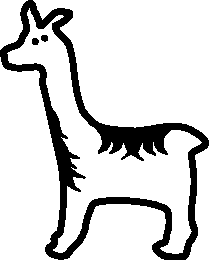
\includegraphics[height=1in]{llama.pdf}
\end{center}

Louie Llama is rather radical for a llama---he doesn't mind being
ROTATED one bit.

\mynewpage



\begin{question}
  Let's take Louie Llama for a walk.
  \begin{enumerate}
  \item Draw an obtuse, non-right, scalene triangle whose sides are
    between $50$ and $300$ millimeters in length. Use a RULER and a
    PROTRACTOR to measure sides and the angles. LABEL side-lengths and
    angle measures.
  \item Now, use your imagination (and artistic skills) to visualize
    Louie Llama starting at the middle of one side and walking around
    the triangle, ALWAYS keeping his FEET facing the sides. At EACH
    VERTEX of the triangle, LABEL the angle through which Louie Llama
    turns.
  %% \item Write a \snap\ SCRIPT that demonstrates that your answers from
  %%   part (b) are correct. \textbf{You should start Louie Llama out in the
  %%   MIDDLE of a side.}  Show off your work by giving screenshots of
  %%   your SCRIPT and your STAGE.
  \end{enumerate}
  \begin{freeResponse}
    \begin{enumerate}
    \item Here it is:
      \begin{center}
        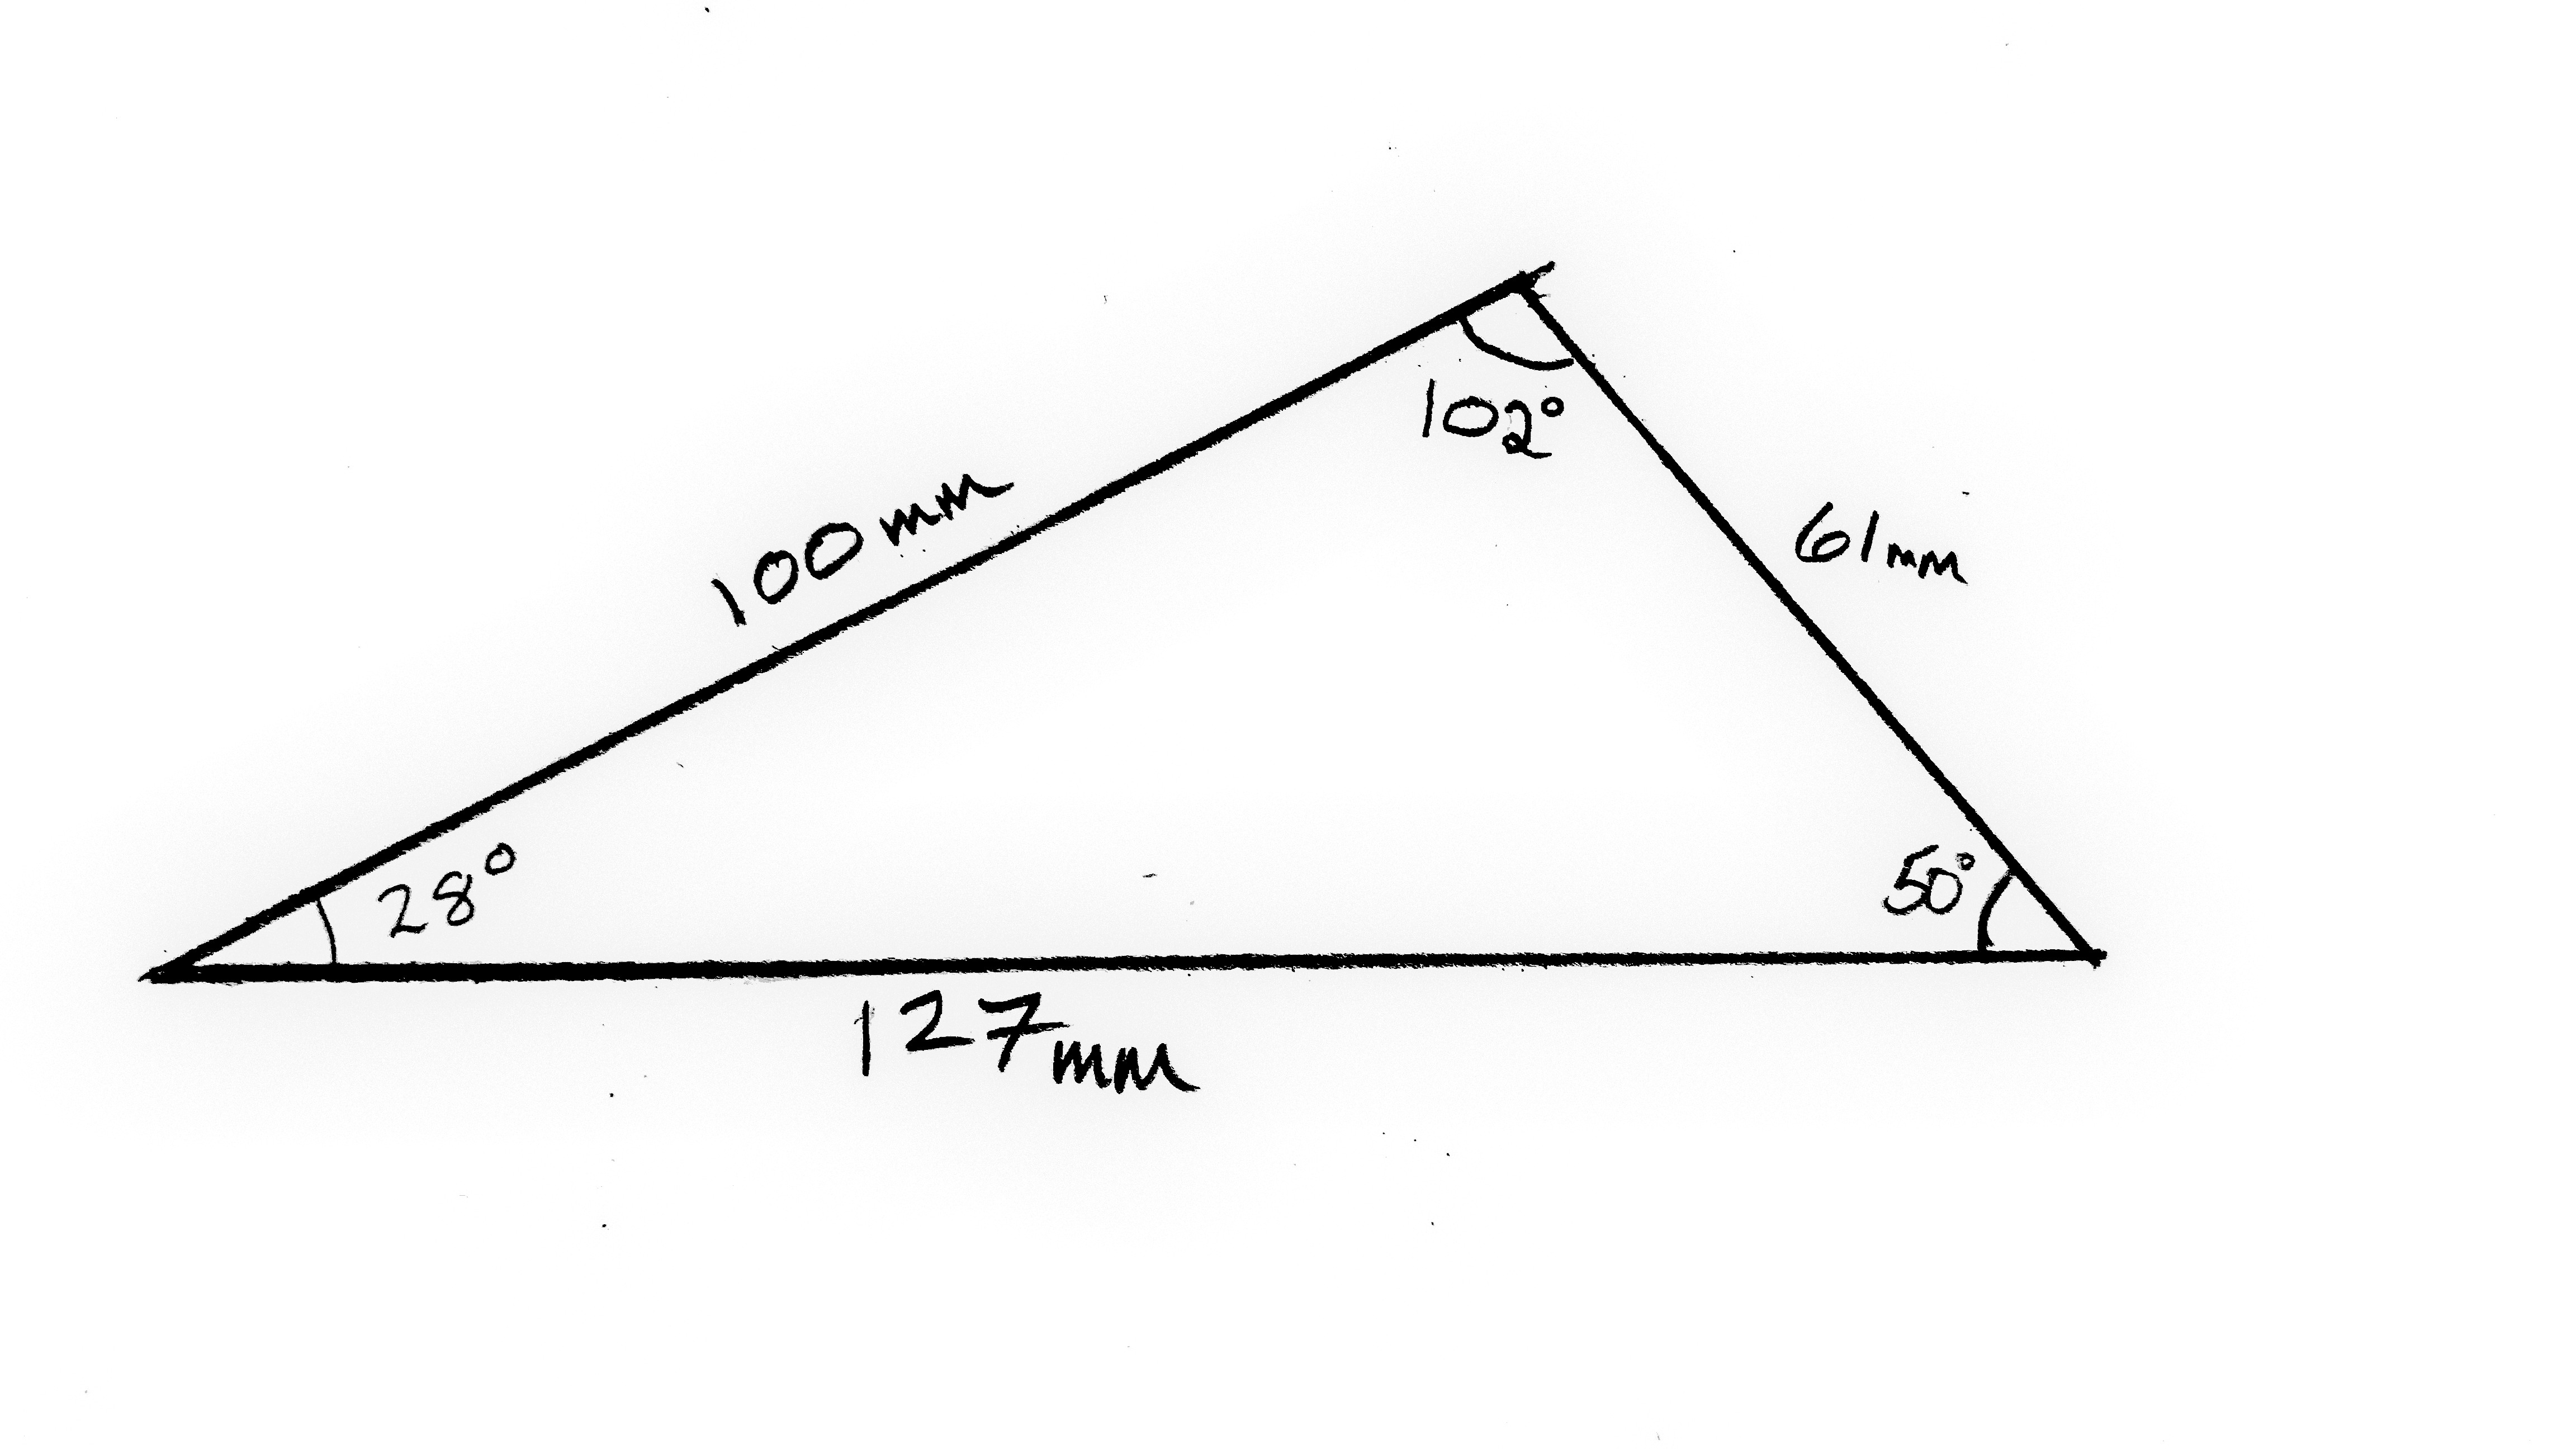
\includegraphics[width=.4\textwidth]{specificTri.jpg}
      \end{center}
    \item Here it is:
      \begin{center}
        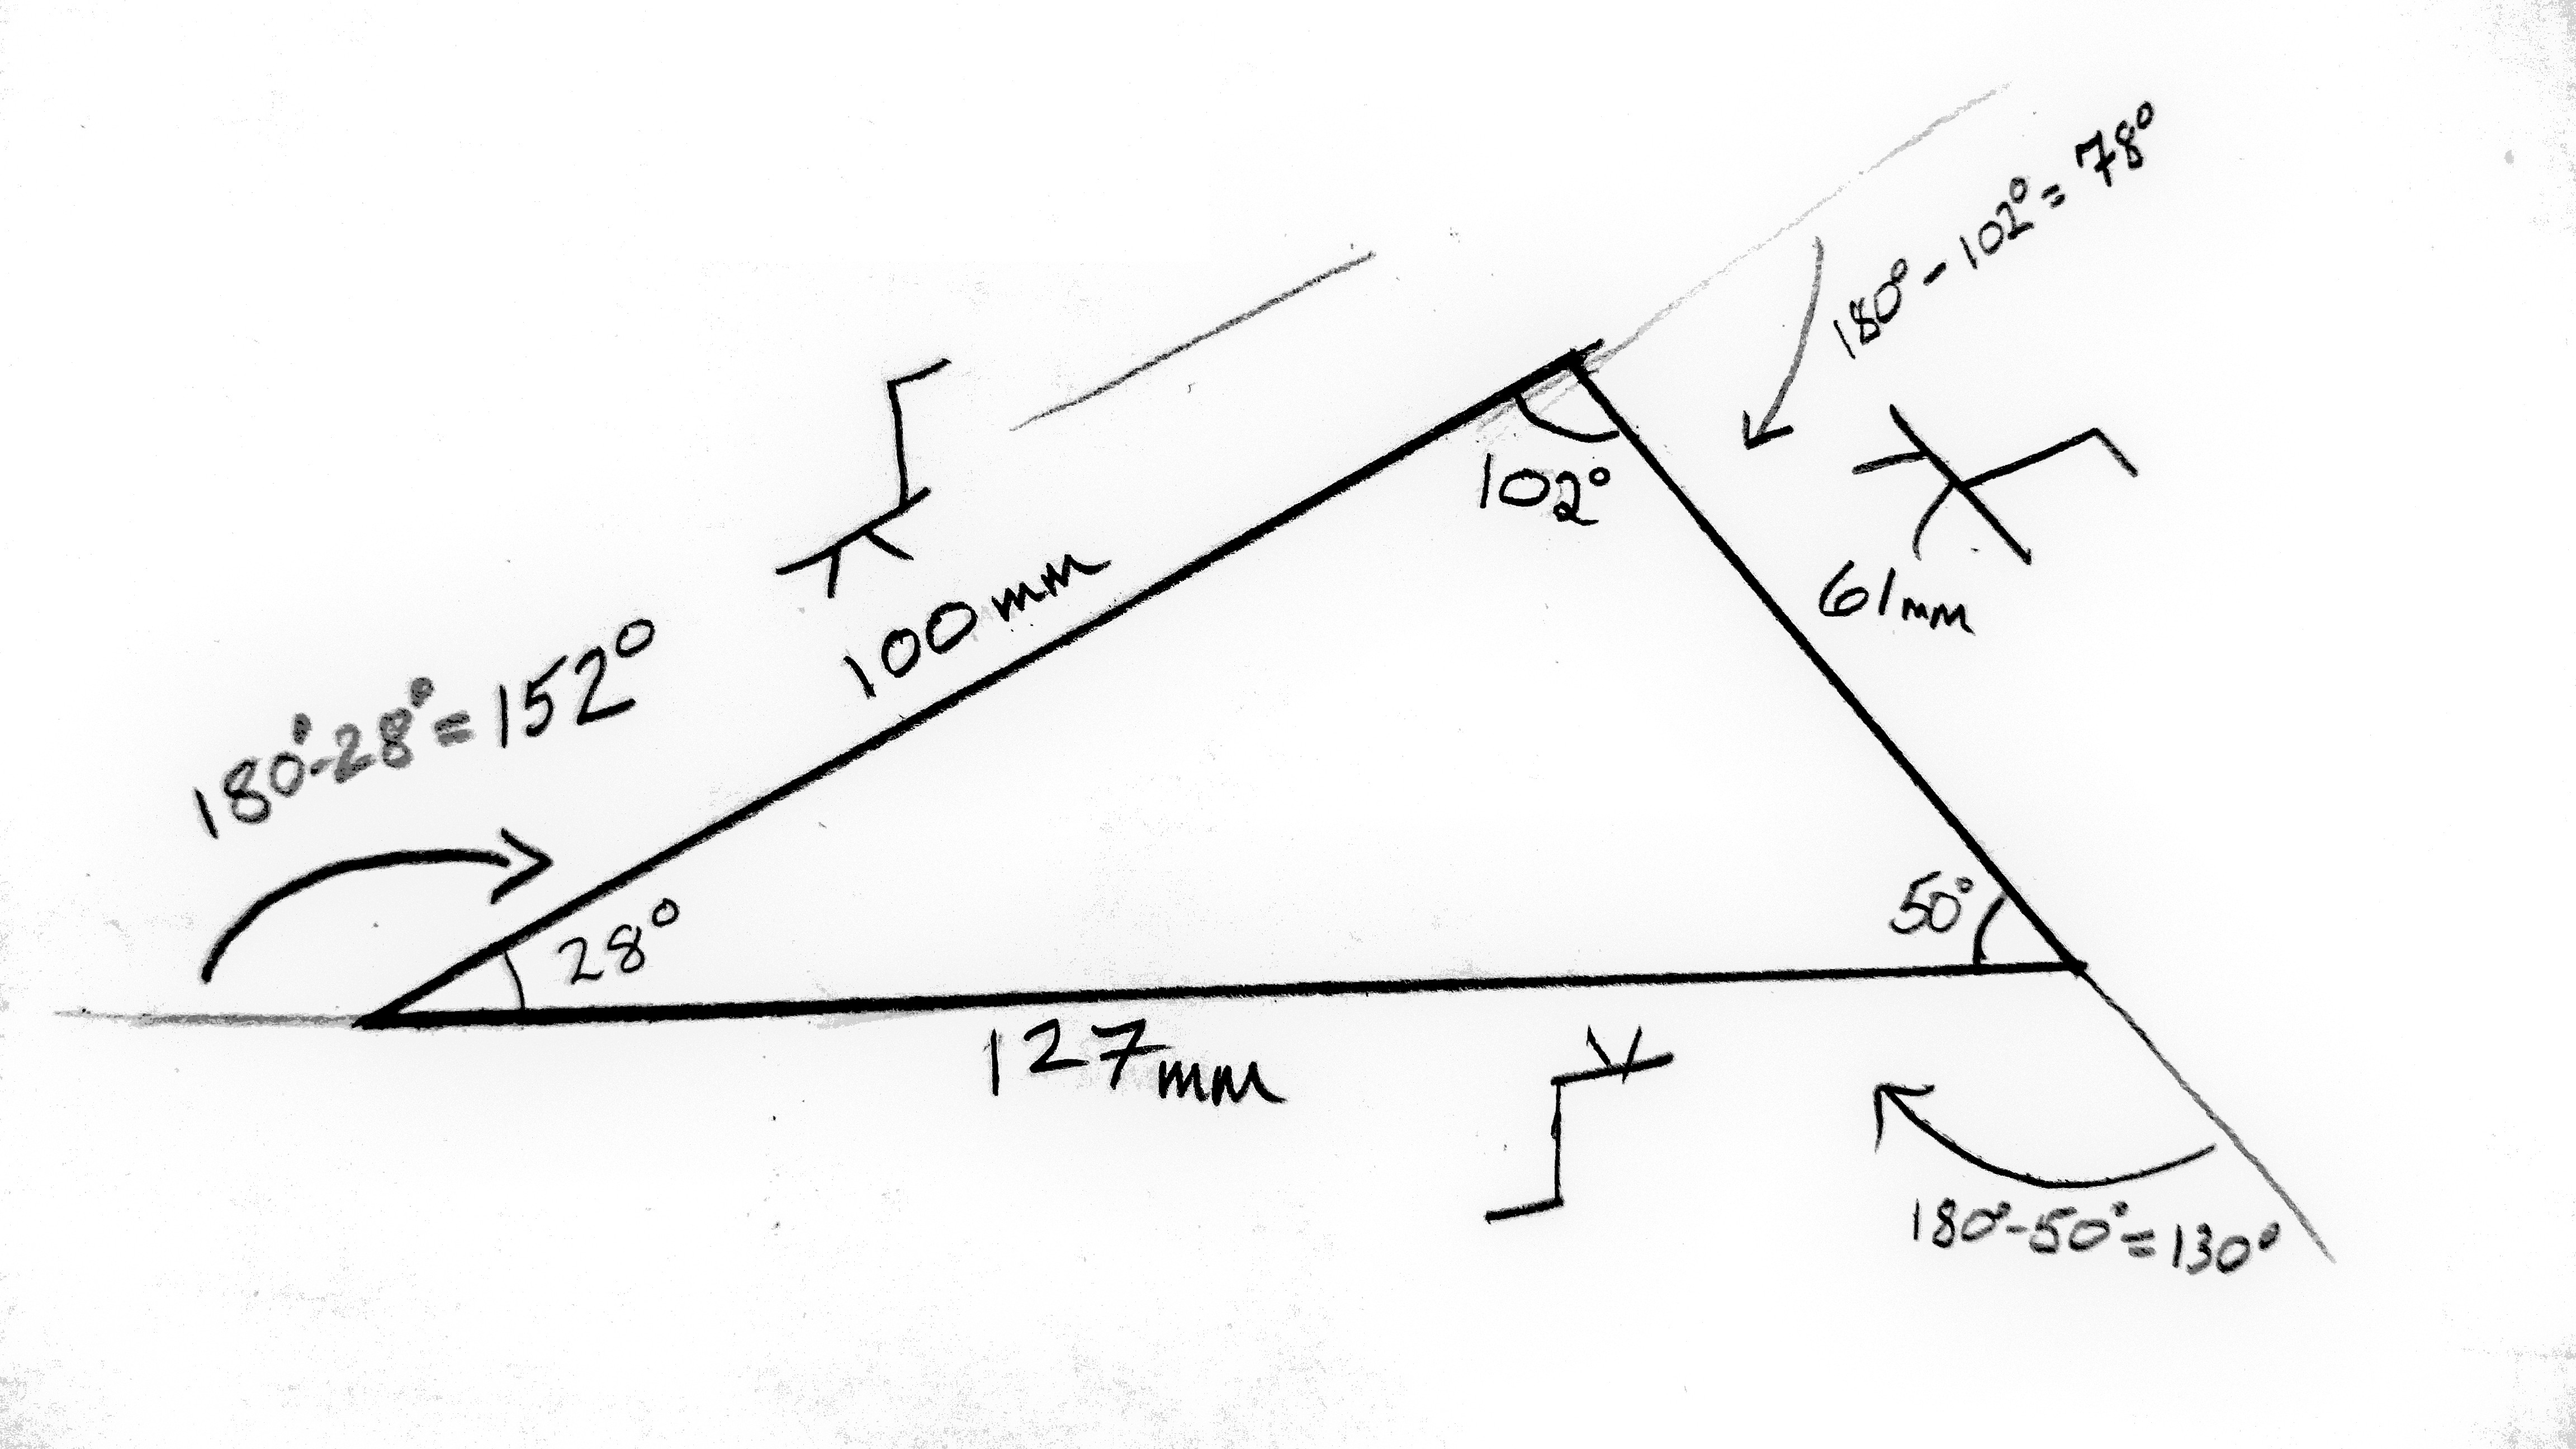
\includegraphics[width=.4\textwidth]{llamaAndSpecificTri.jpg}
      \end{center}
    %% \item Here is my script and stage for the pentagon:
    %%   \begin{center}
    %%     \raisebox{-.2\height}{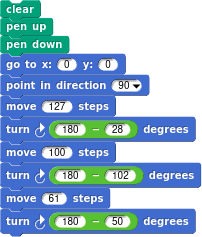
\includegraphics{SCRIPTllamaWalk.png}}
    %%     \qquad
    %%     \fbox{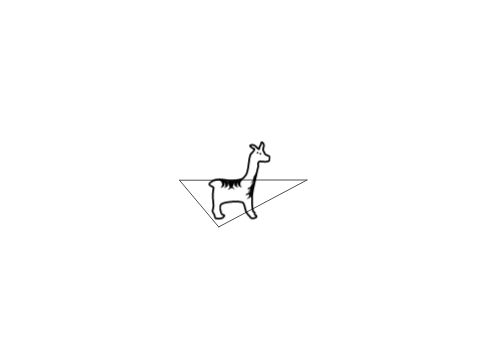
\includegraphics[width=.4\textwidth]{STAGEllamaWalk.png}}
    %%   \end{center}
      
    \end{enumerate}
  \end{freeResponse}
\end{question}

\mynewpage


\begin{question}
  Let's take Louie Llama for a more general walk.
  \begin{enumerate}
  \item Draw some non-right scalene triangle, but this time label the
    angles $\alpha$, $\beta$, and $\gamma$. Again, imagine Louie Llama
    starting at the middle of one side and walking around the
    triangle, ALWAYS keeping his FEET facing the sides. At EACH VERTEX
    of the triangle, LABEL the angle through which Louie Llama turns.
  \item In TOTAL, how much did Louie Llama turn? Give a very brief and quick explanation.
  \item Write an equation where the right-hand side is Louie Llama's
    total rotation and the left-hand side is the sum of each rotation
    around the angle. SOLVE for $\alpha+\beta+\gamma$.
  \end{enumerate}
  \begin{freeResponse}
    \begin{enumerate}
    \item Here it is:
      \begin{center}
        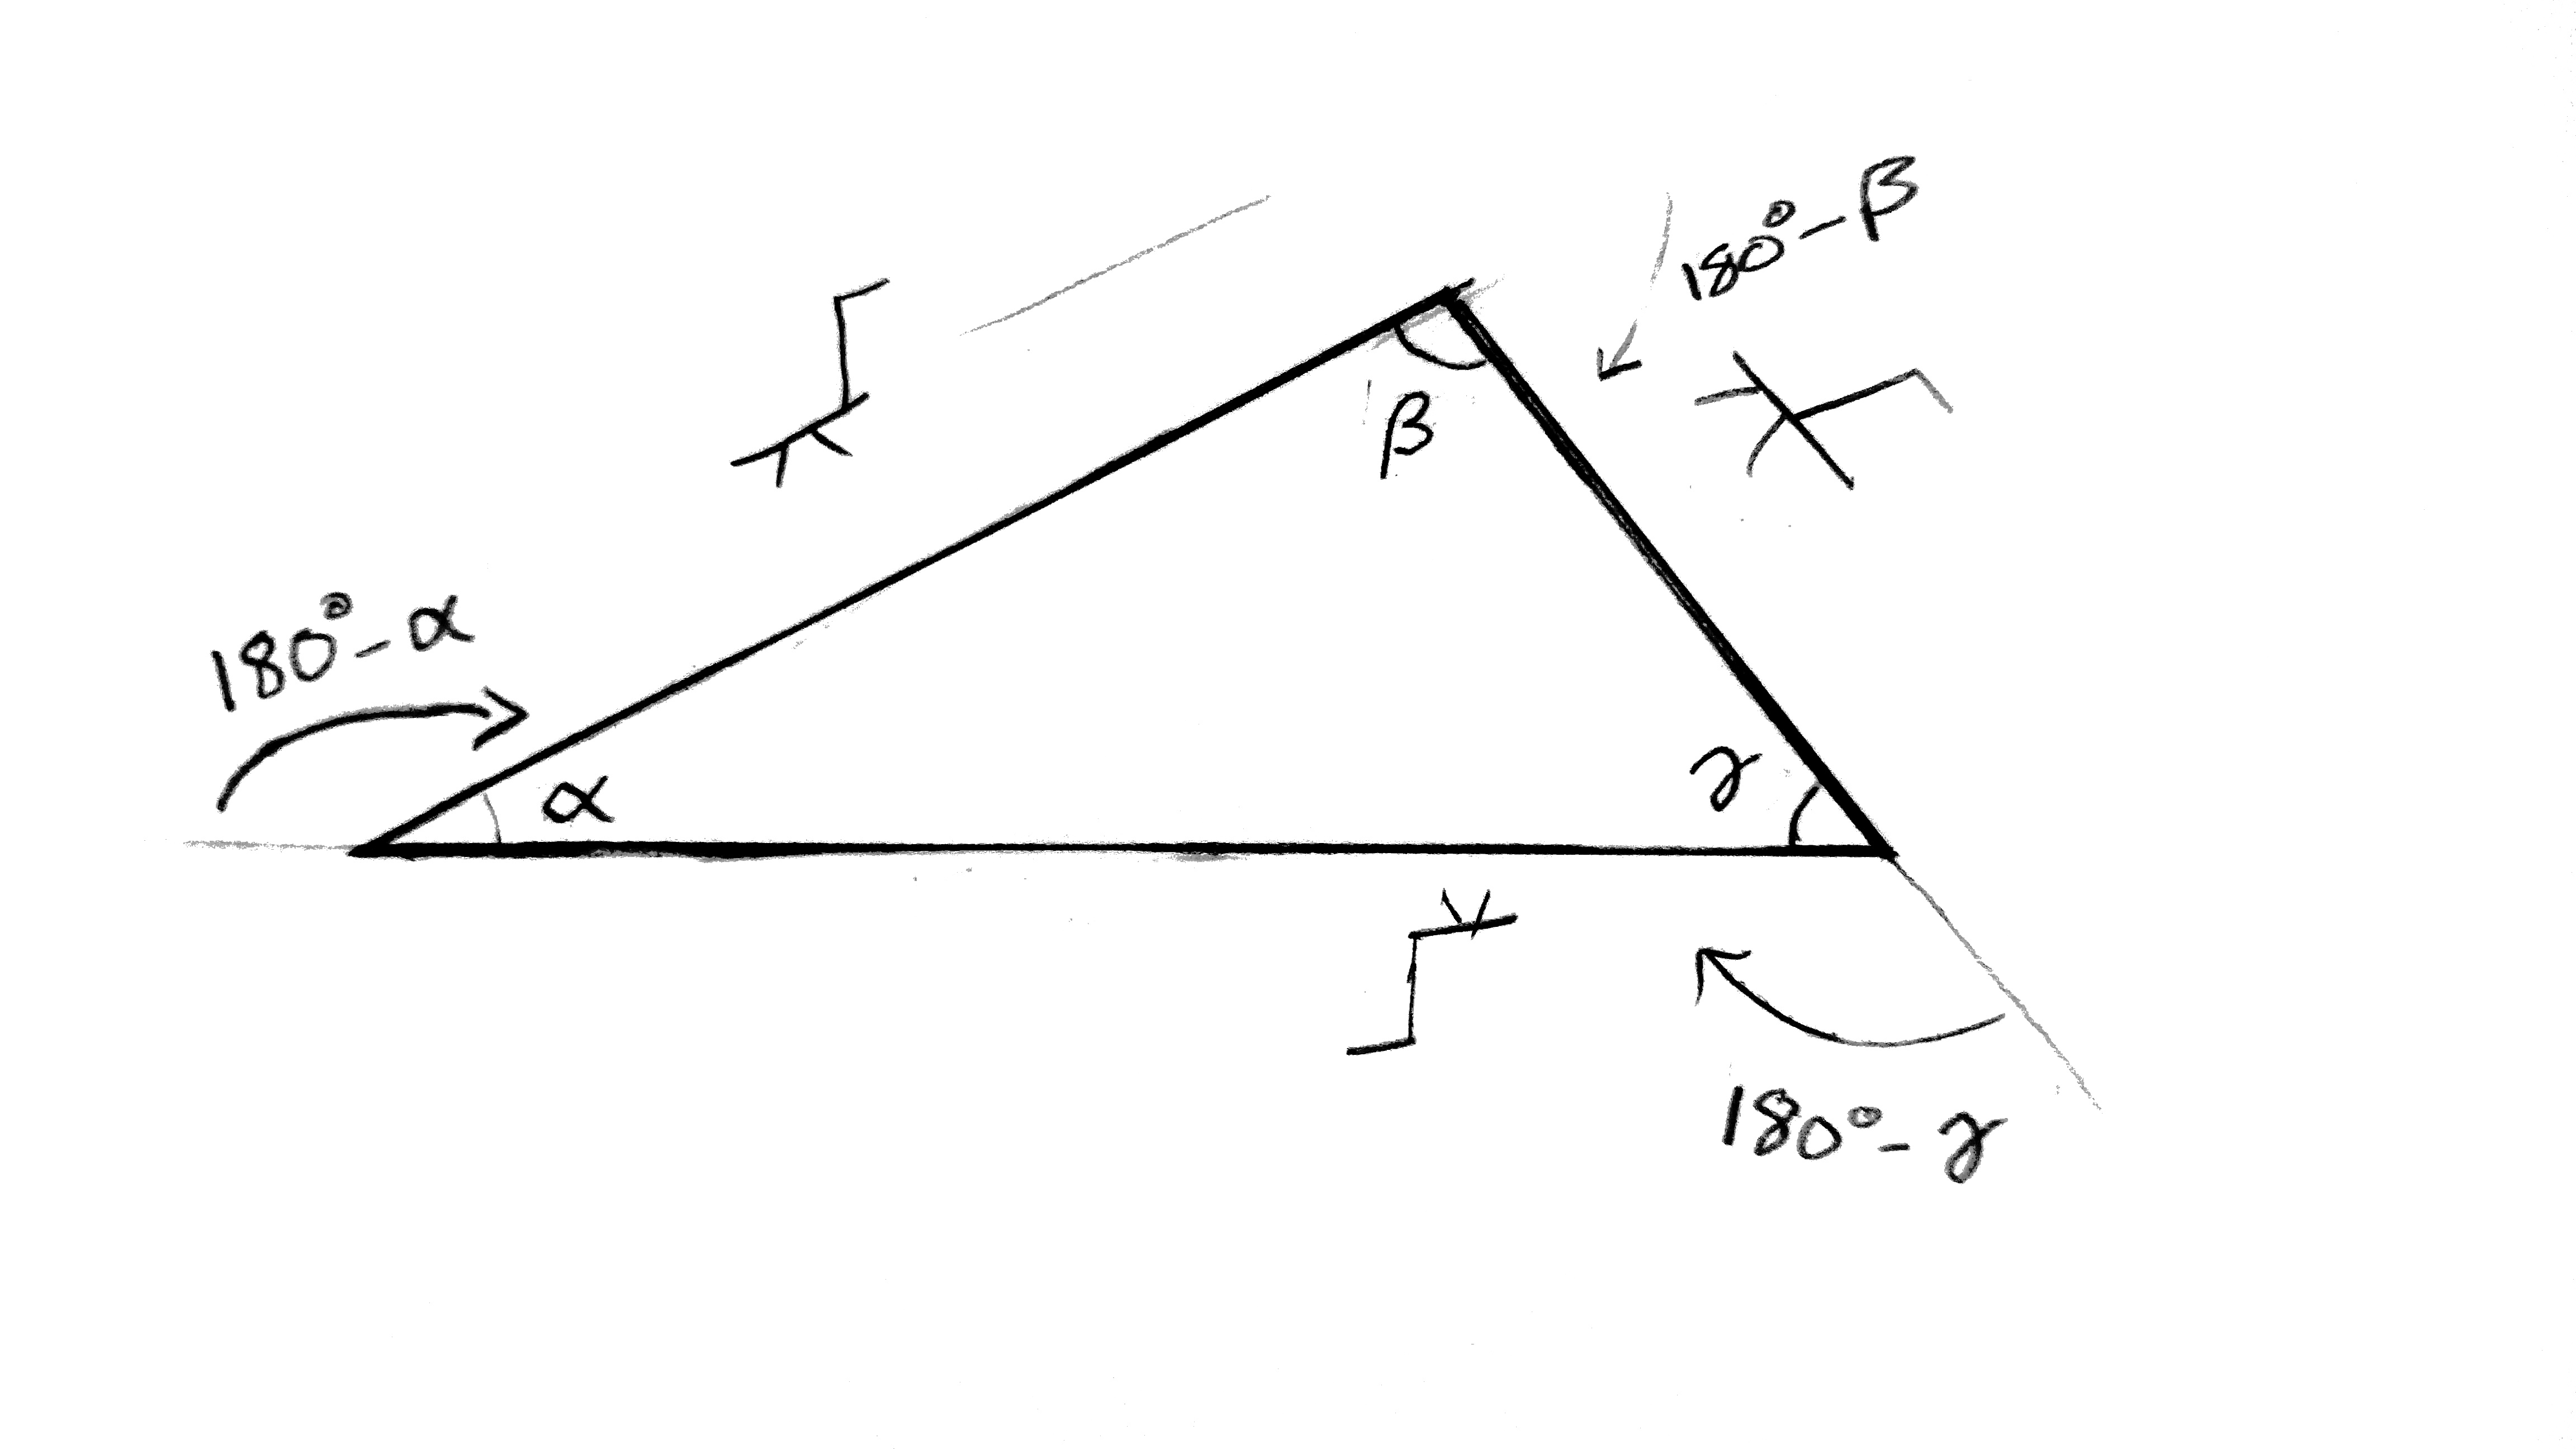
\includegraphics[width=.4\textwidth]{generalTriAndLlama.jpg}
      \end{center}
    \item I can SEE he turned $360^\circ$!
    \item Write
      \[
      \underbrace{360}_{\text{whole turn}} = \underbrace{180-\alpha}_{\text{first turn}} + \underbrace{180-\beta}_{\text{second turn}} + \underbrace{180-\gamma}_{\text{third turn}}
      \]
      Solving for $\alpha + \beta + \gamma$, we have
      \[
      \alpha + \beta + \gamma = 180.
      \]
    \end{enumerate}
  \end{freeResponse}
\end{question}

\mynewpage


\begin{question}
  Let's walk Louie Llama around other shapes and figure stuff
  out. Fill in the rest of the table below. As a gesture of
  friendship, I've filled in the top row. SIMPLIFY the bottom row.
  \[
  \renewcommand{\arraystretch}{3}
  \begin{array}{|c||c|c|c|}\hline
    \text{$n$-gon} & \begin{minipage}{1.3in}\center sum of \\ interior angles \end{minipage} &
    \begin{minipage}{1.5in}\center interior angle \\ of a regular $n$-gon\end{minipage} &
      \begin{minipage}{1.5in}\center exterior (turning) angle \\ of a regular $n$-gon\end{minipage} \\\hline\hline
        3 & 180^\circ & 60^\circ  & 120^\circ \\\hline
        4 & & & \\\hline
        5 & & & \\\hline
        6 & & & \\\hline
        7 & & & \\\hline
        8 & & & \\\hline\hline
        n & & & \\\hline
  \end{array}
  \]
  \begin{freeResponse}
    Here's my table:
    \[
  \renewcommand{\arraystretch}{3}
  \begin{array}{|c||c|c|c|}\hline
    \text{$n$-gon} & \begin{minipage}{1.3in}\center sum of \\ interior angles \end{minipage} &
    \begin{minipage}{1.5in}\center interior angles \\ of a regular $n$-gon\end{minipage} &
      \begin{minipage}{1.5in}\center exterior angles \\ of a regular $n$-gon\end{minipage} \\\hline\hline
        3 & 180^\circ & 60^\circ  & 300^\circ \\\hline
        4 & 360^\circ & 90^\circ & 270^\circ \\\hline
        5 & 540^\circ & 108^\circ & 252^\circ \\\hline
        6 & 720^\circ & 120^\circ & 240^\circ\\\hline
        7 & 900^\circ & 128.6^\circ& 231.4^\circ\\\hline
        8 & 1080^\circ& 135^\circ& 225^\circ \\\hline\hline
        n & (n-2)180^\circ  & \frac{(n-2)180^\circ}{n} & 360^\circ - \frac{(n-2)180^\circ}{n}\\\hline
  \end{array}
  \]
  \end{freeResponse}
\end{question}

\end{document}
